\begin{surferPage}[%
משטח מדרגה שישית של לאבס%
]{%
משטח ממעלה שביעית עם 99 נקודות סינגולריות%
}
    אוליבר לאבס
    \textenglish{ (Oliver Labs)}בנה משטח ממעלה שביעית בזמן שעבד על
    עבודת התזה שלו באוניברסיטת מַיינץ בשנת 2004. משטח זה מחזיק עדיין בשיא העולמי למשטחים ממעלה שביעית,
    אך ייתכן כי קיים משטח ממעלה זו שמספר נקודות הסינגולריות שלו מגיע עד $104$
    !
    המשטח של לאבס ניחן בסימטריה של הפטגון משוכלל (התמונה משמאל).
    תכונה זו בולטת לעין כאשר מביטים על המשטח מלמעלה (התמונה מימין):

    \vspace*{-0.3em}
    \begin{center}
      \begin{tabular}{c@{\qquad}c}
        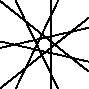
\includegraphics[height=1.5cm]{./../../common/images/labsseptic1.pdf}
        &
        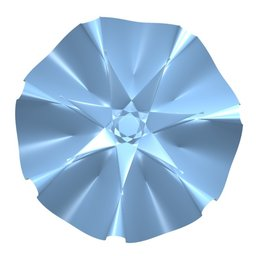
\includegraphics[height=1.5cm]{./../../common/images/labs_septic_von_oben}
      \end{tabular}
    \end{center}
    \vspace*{-0.3em}

    לבניית המשטח, השתמש לאבס במערכת האלגברה הממוחשבת
    {\sc Singular} (אוניברסיטת קייזרסלאוטן) המותאמת היטב
    לביצוע חישובים בגאומטריה אלגברית ונקודות סינגולריות.

    הוא ניצל את העובדה שניתן לחשב באמצעות מערכי מספרים סופיים
    בדרך טבעית. הדבר ידוע לנו מהשעון; 24.00$=$0.00, 24.00 $+ שעה $ 1 הם
    לא 25.00, כי אם 1.00.
\end{surferPage}
